% ============================================================================
% Ligne de niveau de ||a MA + b MB|| = k : cercle de centre G
% Extrait de la fiche : Barycentres et lignes de niveau (classe de 1ere D)
% Necessite \usepackage{tikz} et \usetikzlibrary{calc} (charges par le fichier principal)
% ============================================================================
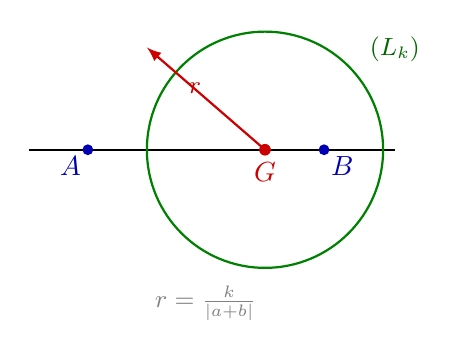
\begin{tikzpicture}[scale=0.75,>=latex]
  \draw[thick] (-1.0,0) -- (5.2,0);
  \draw[thick,green!50!black] (3,0) circle (2);
  \fill[blue!70!black] (0,0) circle (2.6pt) node[below left=-1pt] {$A$};
  \fill[blue!70!black] (4,0) circle (2.6pt) node[below right=-1pt] {$B$};
  \fill[red!80!black] (3,0) circle (2.8pt) node[below=1pt] {$G$};
  \draw[->,red!80!black,thick] (3,0) -- (60:2) node[midway,above left=-2pt,font=\small] {$r$};
  \node[green!40!black,font=\small] at (5.2,1.7) {$(L_k)$};
  \node[font=\small,gray] at (2.0,-2.6) {$r=\frac{k}{|a+b|}$};
\end{tikzpicture}
